\chapter{CoAP resource module} \label{resourcemodule}

Nu we genoeg kennis hebben over Drupal en CoAP en een CoAP library ter beschikking hebben, kunnen we overgaan tot de uiteindelijk te ontwikkelen module. Het is deze module die een eindgebruiker zal installeren. Ze biedt dan de mogelijkheid om op een gebruiksvriendelijke en dynamische manier sensoren te bekijken en beheren van op de Drupal website, en dit zonder technische kennis nodig te hebben van het CoAP protocol of programmatie in Drupal. We bekijken eerst globaal wat de module concreet moet aanbieden. Daarna bekijken we hoe de module zal opgebouwd worden. Eens we dit weten, kunnen we overgaan tot de verschillende versies van de ontwikkelde module en de implementatie ervan.

\section{Architectuur}
In deze paragraaf bespreken we de architectuur van de module en hoe die inpast in het Drupal systeem. We behandelen tevens ook enkele belangrijke aspecten die in rekening werden gebracht. Vervolgens lichten we enkele belangrijke onderdelen van de module.\\
De architectuur wordt weergegeven in figuur \ref{fig:architectuur}. De acties aangeduid met een gekleurd bolletje gebeuren altijd bij een request, de acties aangeduid met een leeg bolletje zullen pas gebeuren wanneer geen geldige waarde uit de databank kan worden gehaald(Zie paragraaf \ref{caching}).\\
We overlopen de opeenvolgende stappen bij een request aan de hand van figuur \ref{fig:architectuur}:
\begin{enumerate}
\item De client start een periodiek poll naar de webserver waarop Drupal draait. Deze poll gebeurt onder vorm van een AJAX call.
\item De CoAP Resource module voert een query uit op de databank om een geldige waarde op te vragen indien die aanwezig is.
\item De databank stuurt een resultatenset terug die een geldige waarde bevat, of leeg is indien er geen geldige waarde meer is.
\item In deze stap zijn er twee mogelijkheden:
\begin{itemize}
\item Indien er een geldige waarde aanwezig is in de databank, wordt deze teruggestuurd naar de client als antwoord op de AJAX call. De request eindigt dan hier.
\item Indien er geen geldige waarde aanwezig is in de databank, wordt een beroep gedaan op de CoAP library module om een nieuwe waarde op te vragen aan de resource. 
\end{itemize}
Dit mechanisme zorgt ervoor dat de resource niet onnodig belast wordt (Zie paragraaf \ref{caching}).
\item De CoAP library module stuurt een CoAP GET request naar de resource.
\item De resource stuurt zijn waarde terug op in een response bericht als antwoord op de GET request.
\item De CoAP library roept een hook op die de CoAP Resource module ge\"{i}mplementeerd heeft, om die ervan op de hoogte te brengen dat er een waarde is binnengekomen.
\item De hook zal ervoor zorgen dat de nieuwe, ontvangen waarde opgeslagen wordt in de databank.
\item Uiteindelijk wordt de waarde ook teruggestuurd naar de client die de request heeft gestart.
\end{enumerate}
\begin{figure}
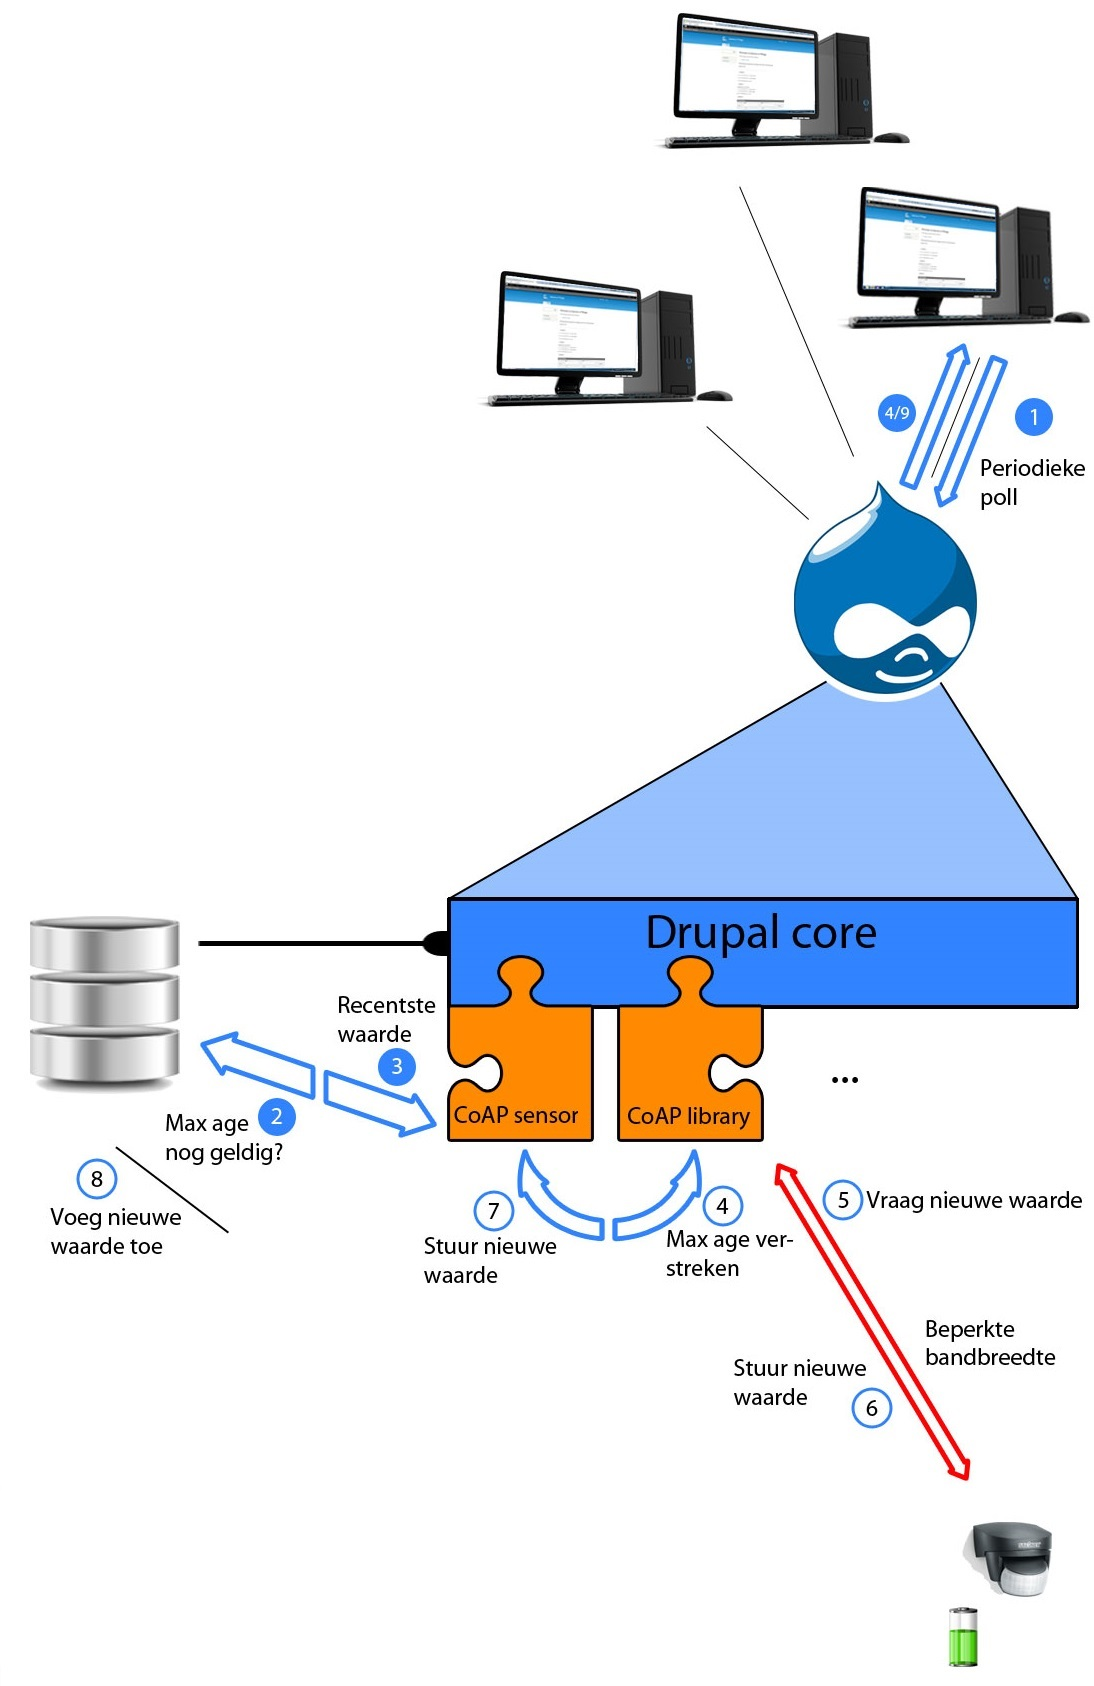
\includegraphics[width=1\textwidth]{fig/architectuur}
\caption{Architectuur van de CoAP resource module in Drupal}
\label{fig:architectuur}
\end{figure}

\subsection{Functionaliteit}

De bedoeling van deze module is de eindgebruiker in staat te stellen om gemakkelijk sensoren te beheren op zijn/haar website. Belangrijk hierbij is dat elke Drupal gebruiker die een website maakt, deze kan gebruiken zonder extra kennis nodig te hebben over het CoAP protocol. Ook is het niet de bedoeling dat de eindgebruiker zelf nog moet programmeren in Drupal om de module te kunnen gebruiken. Kortom, de module moet out-of-the box werken en zoveel mogelijk omvatten wat mogelijk is met CoAP sensoren.\\
Concreet houdt dit onder andere in dat bij installatie van de module enkele content types mee worden ge\"{i}nstalleerd. Het betreft hier een content type voor een enkele CoAP resource en een content type voor een CoAP device waarop meerdere resources zitten. Ook hier werd weer modulair gewerkt, de resources worden bij een CoAP device aangegeven onder vorm van het content type CoAP resource. Deze content types zorgen ervoor dat de gebruiker slechts met enkele muisklikken het resources en devices kan toevoegen en onmiddellijk kan beginnen met het beheren en bevragen van de resources. Verder worden bij installatie ook alle benodigde databanktabellen gecre\"{e}erd.\\

De configuratie die de gebruiker moet doen zoals bijvoorbeeld het toevoegen van een resource, moet gebruiksvriendelijk verlopen. Hiervoor wordt gebruik gemaakt van resource discovery. In het geval van een CoAP device hoeft de gebruiker enkel het IPv6-adres ervan op te geven. Aan de hand van resource discovery wordt dan een lijst gegenereerd van resources. Wanneer de gebruiker op een resource klikt, krijgt die een visuele representatie van het content type CoAP resource.\\
Wanneer de gebruiker een enkele resource wil toevoegen, hoeft die enkel de URI van de resource op te geven. Deze bestaat uit een IPv6-adres en een URI-path, gescheiden door een '/'. De module zal aan de hand van een specifieke resource discovery voor deze resource, de overige informatie en parameters van de resource ophalen en opslaan in de databank. De resource wordt bij de discovery gespecifieerd door een Uri-Query optie toe te voegen aan het CoAP pakket met een waarde onder de vorm van 'href=/resource'. De parameters bestaan onder andere uit het content type dat de resource teruggeeft (plain text, JSON, XML, ...), of de resource al dan niet observable is, enzovoort...\\

Eens de gebruiker de gewenste resources heeft toegevoegd aan zijn/haar website, is het de bedoeling dat de 4 REST-methodes GET, PUT, POST, DELETE kunnen uitgevoerd worden, de gebruiker zal ervan op de hoogte gebracht worden wanneer een methode niet ondersteund wordt. Naast deze methodes kan een sensor ook nog observable zijn (zie hoofdstuk \ref{CoAP}), de gebruiker moet dus ook in staat gesteld worden om notificaties te ontvangen van een resource. Ook wanneer een gebruiker de website verlaat moet het mogelijk zijn de observe te laten doorlopen.

\subsection{Belangrijke aspecten}

Deze module werd ontworpen met het oog op bepaalde aspecten waarmee rekening moet worden gehouden. We sommen enkele van de belangrijkste op.

\subsubsection{Modulariteit}
Een van de grote troeven van Drupal is de modulariteit die aangeboden wordt. Het is dan ook van uiterst belang dat onze module dit principe niet verbreekt, maar juist doorzet. In hoofdstuk \ref{coaplibrary} zagen we al hoe een aparte CoAP library ontwikkeld werd. Dit heeft als gevolg dat elke Drupal gebruiker de kans heeft gebruik te maken van de library en dus zelf een module zou kunnen bouwen gelijkaardig aan de onze.\\
Dit geldt ook voor deze module die we nu bespreken, deze is ook bruikbaar voor elke gebruiker die dat wil. Naast het installeren van de CoAP library en deze module, hoeft de gebruiker niets extra te doen om deze module te gebruiken. Databanktabellen worden gecre\"{e}erd en content types worden ge\"{i}nstalleerd, zonder dat de gebruiker daar iets hoeft voor te configureren.\\
Onze module heeft zo ook enkele modules nodig die de gebruiker eerst moet installeren. Drupal zal hierbij automatisch de gebruiker aangeven welke modules eerst moeten worden ge�nstalleerd. Het betreft de volgende modules:
\begin{itemize}
\item Background process: Deze module maakt namelijk gebruik van achtergrondprocessen (bvb voor observe)
\item CoAP library: onze eigen geschreven module die instaat voor alle CoAP communicatie
\item Entity: Een veelgebruikte module (wordt namelijk opgenomen in Drupal 8) om data in een vaste en gemakkelijk te behandelen structuur te gieten
\item Node reference: Een module die gebruikt wordt om in een bepaalde node te verwijzen naar andere nodes
\end{itemize}

\subsubsection{Minimalisatie van netwerkbelasting}
Mogelijks zijn meerdere gebruikers van een Drupal website ge\"{i}nteresseerd in een observable resource. Het is niet aanvaardbaar dat de netwerkbelasting zou stijgen met het aantal ge\"{i}nteresseerden. Daarom gedraagt Drupal zich eigenlijk als intermediaire server voor de eindgebruikers. Er wordt namelijk maar \'{e}\'{e}n observe uitgevoerd door Drupal, ongeacht het aantal gebruikers dat ge\"{i}nteresseerd is. De notificaties worden op de server in de databank gestopt en het zijn deze waarden waarop de gebruikers uiteindelijk pollen.\\
Bovendien zorgt dit voor een vorm van controle over verkeer naar de resources, de gebruikers van de website kunnen namelijk niet zelfstandig CoAP praten met de resources. Een voorbeeld hiervan is de demo van de module op onze website. Enkel ingelogde gebruikers zijn in staat een observe uit te voeren. Dit om te vermijden dat gelijk wie een observe kan starten, men kan namelijk vergeten de observe af te sluiten, waardoor de databank meer en meer opgevuld wordt.

\subsubsection{Asynchroniteit}
In een eerste fase van deze module werd er gebruik gemaakt van een formulier. Bij het indienen van dit formulier, werd eerst de request om de waarde op te halen uitgevoerd en dan gewacht op de response om de nieuwe pagina op te bouwen. Het spreekt voor zich dat dit geen goed oplossing is, daar de gebruiker zal moeten wachten op de pagina wanneer de communicatie traag is of misloopt, de gebruiker kan snel het idee krijgen dat er geen verbinding meer is met de website.\\

In hoofdstuk \ref{Drupal} zagen we dat een mogelijke oplossing het gebruik van jQuery is. In deze situatie is jQuery echter geen goede optie, daar jQuery de databank van Drupal niet zomaar kan manipuleren. Hiervoor zouden een connectiestring, wachtwoord en dergelijke gegevens nodig zijn, en jQuery van die informatie voorzien is een grote bedreiging voor de veiligheid, bovendien zou dit een oplossing zijn met een zeer sterke koppeling, wat nooit een goed idee is.\\
De gebruikte oplossing illustreert alweer de voordelen van een open source platform met een uitgebreide community. Er is namelijk al een Background Process module gemaakt in het verleden, het zou dus zonde zijn om hier niet dankbaar gebruik van te maken. Zoals de naam suggereert, biedt de Background Process module de mogelijkheid om achtergrondprocessen op te starten. Deze draaien op de achtergrond op de server en storen dus geen andere processen zoals het opbouwen van een pagina voor de gebruiker, waardoor de gebruiker dus niet geconfronteerd wordt met lange wachttijden.\\
Sterker nog, er is ook een functie voorzien om een HTTP GET-request uit te voeren, waarbij je een callback-functie opgeeft. Wanneer er een response is, zal dus automatisch de opgegeven functie opgeroepen worden met de response als argument. Deze functie zal dus goed van pas komen in de eerste versie van de module, die gebruik maakt van een HTTP/CoAP-proxy. Deze wordt beschreven later in dit hoofdstuk.

\subsubsection{Strategie bij ontvangst van waarden}
\paragraph{Push-strategie:}

De mooiste oplossing en tevens degene met het minste aandeel aan overhead, is een oplossing waarbij de server zelf op eigen initiatief data kan sturen naar de client. Hierbij is dan geen polling-mechanisme nodig door de client, wat de netwerkbelasting drastisch verlaagt en de verantwoordelijkheid verschuift naar de server.\\
Om een push-strategie te verwezenlijken werd een uitgebreide literatuurstudie van node.js uitgevoerd. Node.js is een javascript-library die je in staat stelt bi-directioneel verkeer te verwezenlijken. Hierbij wordt gebruik gemaakt van kanalen die worden opgezet, zo'n kanaal kan dan door beide partijen gebruikt worden.\\
Concreet zou het in de context van deze masterproef mogelijk zijn om met node.js een JavaScript-functie op te roepen bij de client op initiatief van de server.\\

Er is meermaals gepoogd dit te realiseren, maar de summiere documentatie van node.js laat op sommige vlakken te wensen over. Zo zijn we er niet in geslaagd documentatie te vinden over het opzetten van een eigen kanaal of een bestaand kanaal te gebruiken.\\
Bovendien is het nodig voor node.js om een extra server te draaien waarlangs het verkeer moet passeren. Aangezien het vaak niet mogelijk is om de shell van de webserver te gebruiken in een free-hosting omgeving, is dit een erg groot nadeel. Er bestaan wel servers die je kan gebruiken, maar dit tegen betaling. Wij, als ontwikkelaar van de module, kunnen niet verwachten dat een eindgebruiker een extra server ter beschikking heeft of dat zelfs wilt. Het is de bedoeling dat onze module zo veel mogelijk out-of-the-box bruikbaar is.\\

De conclusie is dat wij geopteerd hebben geen gebruik te maken van node.js en dus ook niet van een push-strategie.

\paragraph{Pull-strategie: }

Aangezien een push-strategie niet of moeilijk kan gebruikt worden, hebben wij gekozen voor een pull-oplossing.\\

Uiteraard was de eerste reactie gebruik te maken van de Drupal-community en dus te zoeken in de vele modules die beschikbaar zijn. Er is tot op heden geen module geschreven door iemand anders in de Drupal-community dat ons probleem behandelt. De inspiratie voor de uiteindelijke oplossing werd wel gehaald uit een bestaande module, namelijk de Block Refresh-module.\\
Deze laatste maakt gebruik van jQuery en AJAX calls om periodiek de inhoud van een block te refreshen, waarbij je zelf de lengte van de periode kan bepalen. In jQuery loopt een timer die periodiek een JavaScript-functie oproept. In deze functie wordt dan een AJAX call uitgevoerd naar de Drupal server, die op zijn beurt een antwoord terug stuurt.\\

Wij hebben geopteerd het mechanisme licht te wijzigen in plaats van de module zelf te gebruiken. Aan de oorzaak van deze beslissing liggen drie redenen:
\begin{itemize}
\item Wij wensen de content slechts aan te passen wanneer nodig. Dit wil zeggen, wanneer een nieuwe waarde is binnengekomen. Bovendien hoeft niet alle content vernieuwd te worden, dit doet de Block Refresh module wel.
\item De configuratie van de periode voor het vernieuwingsinterval is in onze ogen relatief omslachtig. De gebruiker moet al een configuratievenster openen om het interval te wijzigen, wat wachttijden met zich meebrengt. Het zal blijken dat in onze uiteindelijke module het interval snel en gemakkelijk te wijzigen is. 
\item In de uiteindelijke module zal geen blocks meer gebruiken, maar content types. Dit maakt het gebruik van de Block Refresh module zelfs onmogelijk.
\end{itemize}

De aangepaste methode gaat als volgt: Wanneer de pagina geladen wordt bij de client, start een timer die periodiek een AJAX call uitvoert naar de Drupal server. De gebruiker kan hierbij bepalen hoe lang die periode moet zijn. Op de Drupal server is dan een AJAX callback functie gedefinieerd aan de hand van de hook hook\_menu(). Deze hook wordt gebruikt om menu items toe te voegen aan de site en om AJAX callbacks te definieren. Alle output die gegenereerd wordt in deze callback wordt als antwoord teruggestuurd op de AJAX callback.\\

Wat de callback terugstuurt en hoe die inhoud wordt verwerkt, verschilt per versie van onze module. Dit zal dan ook besproken worden in de gepaste paragrafen.

\subsubsection{Caching}\label{caching}
Een bericht kan een maximum levensduur hebben, dit wordt aangegeven met een max-age optie in het bericht. Deze bevat dan een numerieke waarde die aangeeft in seconden hoelang de waarde als geldig mag worden beschouwd. Wanneer deze maximum levensduur overschreden wordt, mag deze waarde niet meer worden gebruikt. Dan moet bij een volgende aanvraag door een gebruiker een nieuwe waarde worden opgehaald van de resource. Bijgevolg wordt een opgehaalde waarde in de databank gestopt. Wanneer de maximum levensduur nog niet overschreden is bij een aanvraag, wordt de waarde uit de databank gehaald. De resource wordt dan dus niet onnodig belast. Dit zorgt er ook voor dat de belasting op een resource niet evenredig stijgt met het aantal gebruikers die er een waarde van willen opvragen.\\
Dit aspect is zeker een van de meer belangrijke omdat verbindingen naar een resource vaak een beperkte bandbreedte kennen. Bovendien bestaat de energievoorziening van sensoren vaak uit een batterij. Het werk dat zo'n sensor moet verrichten, moet dus worden geminimaliseerd.

\subsection{Content-type in de databank}
Onder content-type van de databank verstaan we de definitie van nodige databanktabellen en -kolommen. ----- nog te bekijken

\subsection{Content-types in Drupal}

Bij installatie van de module worden twee content types mee ge\"{i}nstalleerd. We bespreken wat de mogelijkheden ervan zijn en hoe ze eruitzien. Het laten installeren van content types zorgt ervoor dat een Drupal gebruiker op een eenvoudige manier content kan toevoegen, in dit geval onderdelen van een CoAP sensornetwerk. Concreet moet de gebruiker enkel op 'Add content' klikken op zijn/haar Drupal website en het gewenste content type aanklikken. Na invullen van enkele vereiste velden wordt een node gecre\"{e}erd die de content voorstelt.
\newpage
\begin{figure}[h!]
\caption{Content toevoegen door op 'Add content' te klikken.}
\centering
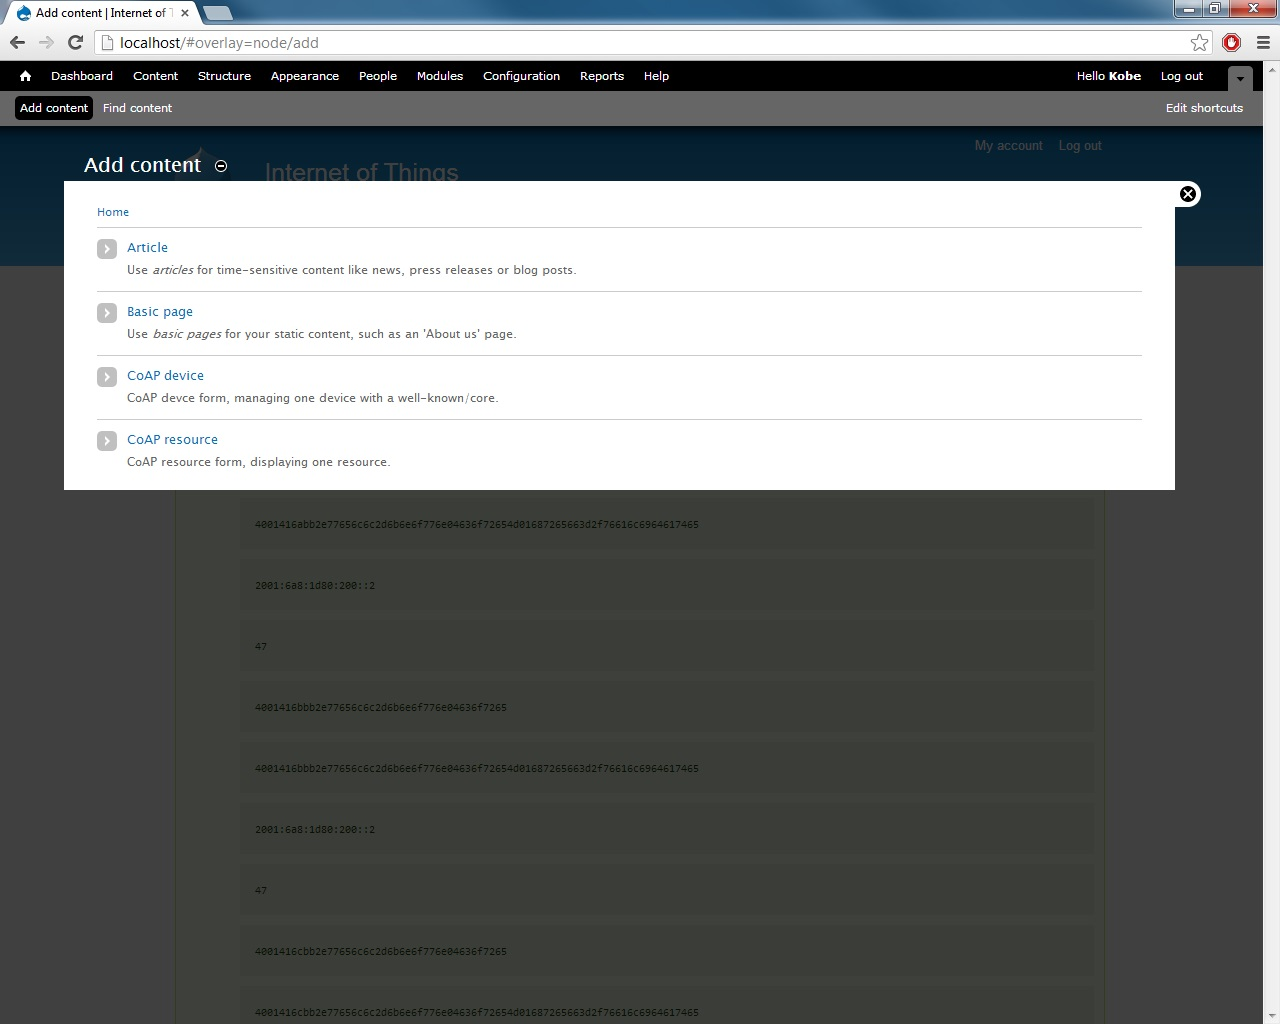
\includegraphics[width=1\textwidth]{fig/add_content}
\end{figure}

\subsubsection{CoAP Resource}
\begin{wrapfigure}{r}{0.6\textwidth}
\vspace{-10pt}
%\hspace{-10pt}
\centering
\label{fig:drupalLogo}
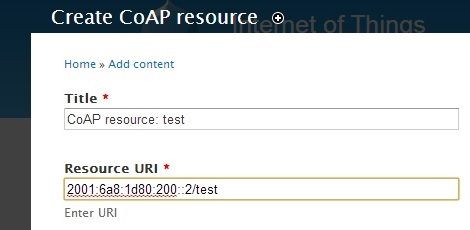
\includegraphics[width=0.6\textwidth]{fig/add_coap_resource}
\vspace{-20pt}
%\hspace{-10pt}
\centering
\caption{Adding content of content type CoAP resource}
\centering
\vspace{-20pt}
\end{wrapfigure}
Dit content type stelt \'{e}\'{e}n resource voor. Bij het toevoegen wordt de URI opgegeven, deze bestaat uit het IPv6-adres van het embedded device waarop de resource is aangesloten en een URI-path. IPv6-adres en URI-path worden gescheiden door een slash ('/'). Een voorbeeld van een door ons vaak gebruikte URI is: 2001:6a8:1d80:200::2/test.\\
Er wordt gevalideerd op de structuur van de URI, wanneer de gebruiker een foute URI opgeeft wordt er een foutmelding getoond en krijgt de gebruiker opnieuw de kans om een geldige URI op te geven. Wanneer de URI gevalideerd is, krijgt de gebruiker de visuele representatie te zien. De gebruiker krijgt nu de kans om de REST-methodes  GET, PUT, POST en DELETE uit te voeren en een observe. Bovendien krijgt de gebruiker een geschiedenis van opvragingen voor deze resource te zien en krijgt ook de kans een grafiek te laten genereren. Voor het type grafiek heeft de gebruiker de keuze uit een lijn-, staaf-, of taartgrafiek.
\begin{figure}[h!]
\centering
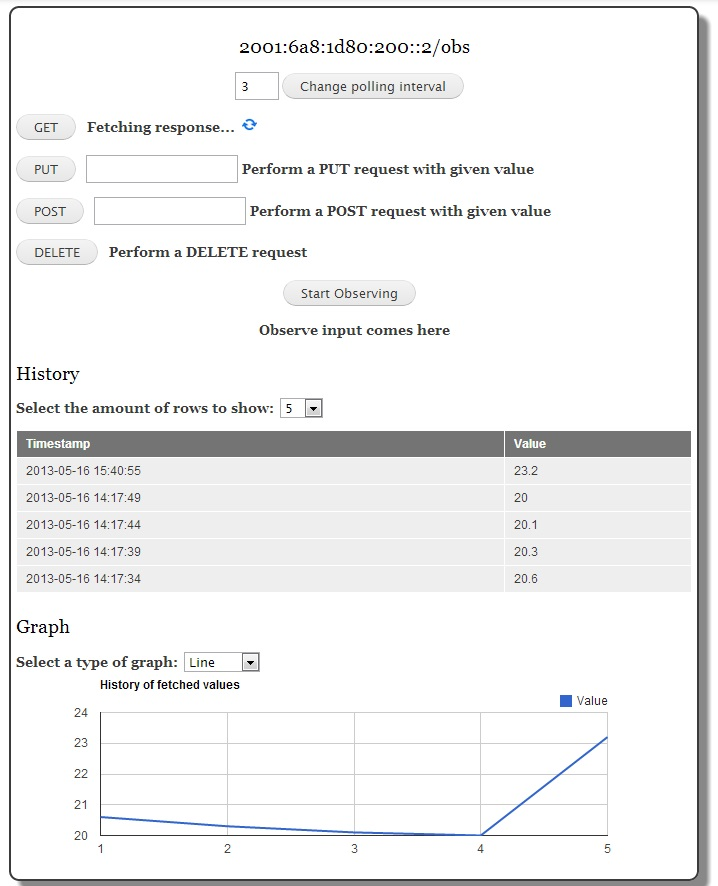
\includegraphics[width=0.8\textwidth]{fig/coap_resource}
\caption{Visuele representatie van het content type CoAP resource.}
\end{figure}

\newpage
\subsubsection{CoAP Device}
\begin{wrapfigure}{r}{0.6\textwidth}
\vspace{-10pt}
%\hspace{-10pt}
\centering
\label{fig:drupalLogo}
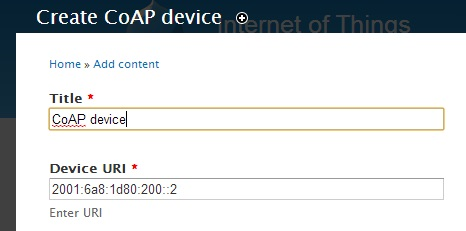
\includegraphics[width=0.6\textwidth]{fig/add_coap_device}
\vspace{-20pt}
%\hspace{-10pt}
\centering
\caption{Adding content of content type CoAP device}
\centering
\vspace{-20pt}
\end{wrapfigure}
Dit content type stelt een volledig embedded device voor waarop \'{e}\'{e}n of meerdere resources zich bevinden. Bij toevoegen van dit content type hoeft de gebruiker enkel het IPv6-adres op te geven. Aan de hand van resource discovery wordt dan een lijst van aangesloten resources opgebouwd en getoond aan de gebruiker. Nu kan de gebruiker doorklikken naar een resource die voorgesteld wordt aan de hand van het content type CoAP resource beschreven in de vorige paragraaf.
\begin{figure}[h!]
\centering
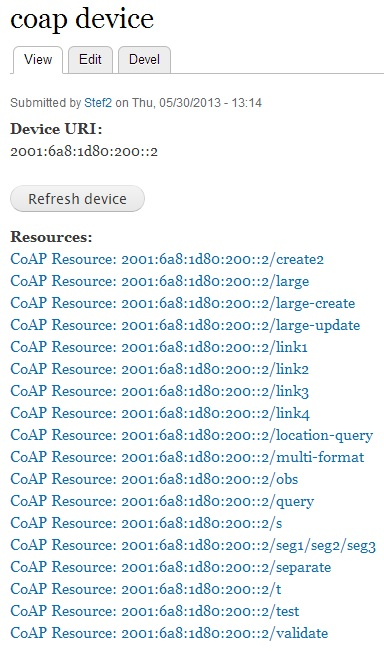
\includegraphics[width=0.6\textwidth]{fig/coap_device}
\caption{Visuele representatie van het content type CoAP device.}
\end{figure}

\section{Evolutie van de module}

\subsection{Temperatuurmodule met HTTP/CoAP-proxy} \label{proxy}
In deze paragraaf wordt besproken hoe de eerste versie van de module werd gemaakt die gebruik maakt van een HTTP/CoAP-proxy. Bovendien wordt ook aangetoond hoe waarden opgeslagen worden in de databank om de geschiedenis van opvragingen bij te houden. Eigenlijk spreken we hier (en in enkele volgende paragrafen) beter van een temperatuurmodule, aangezien deze module slechts \'{e}\'{e}n resource bevraagt. Het betreft een resource die de waarde van een temperatuursensor terugstuurt. Deze resource werd gekozen vanwege de numerieke waarde die teruggestuurd wordt en omwille van het feit dat de resource observable is.\\

De module wordt aan de gebruiker gepresenteerd onder de vorm van een Drupal block. Deze block bevat een HTML-formulier met twee componenten als invoer. Een checkbox die aanduidt of de gebruiker waarden automatisch wil laten ophalen. En een knop die het formulier indient wanneer de gebruiker erop klikt.\\
Wanneer de gebruiker op de knop klikt en de checkbox heeft aangevinkt, worden waarden automatisch opgehaald met een interval gelijk aan de waarde van de max age. Merk op dat het hier nog niet om een CoAP observe gaat, want die is enkel mogelijk met native CoAP, in deze module werken we met een HTTP proxy. Periodiek wordt een HTTP GET-request naar een HTML-pagina uitgevoerd. Wanneer de response ontvangen wordt, wordt de HTML-pagina geparsed, waarna de nuttige informatie in de databank wordt geplaatst. Met jQuery worden dan nieuwe waarden opgehaald en getoond aan de gebruiker.\\

Er is bij deze versie nog geen sprake van achtergrondprocessen waardoor het lang kan duren eer een pagina geladen wordt. Bovendien krijgt de gebruiker enkel een foutmelding te zien wanneer er geen communicatie mogelijk is.

\begin{figure}[h]
\vspace{10pt}
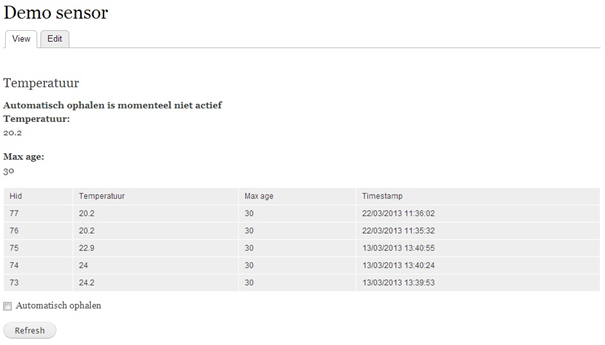
\includegraphics[width=1\textwidth]{fig/TemperatuurModuleHTTPCOAPProxy}
\vspace{-30pt}
\caption{Temperatuurmodule met HTTP/COAP-proxy}
\vspace{-10pt}
\end{figure}

\subsubsection{Proxy}
Als proxy werd de coap.me website gebruikt van iMinds. Deze biedt de mogelijkheid om de notificaties van een embedded device te bekijken in een browser. De website biedt ook de mogelijkheid om door te klikken naar de notificatie om die volledig te bekijken op een pagina.\\

Het is deze laatste pagina die periodiek wordt opgehaald en geparsed. De communicatie vanwege de Drupal-module bestaat dus enkel uit HTTP-communicatie, de proxy verzorgt de nodige CoAP-berichten tussen zichzelf en het embedded device.

\subsubsection{Polling}
In deze eerste versie van de module bestond het antwoord bij de polling uit de volgende velden:
\begin{itemize}
\item Hid: De History ID die een numerieke ID is voor de opgevraagde waarde. Het is tevens de index in de databanktabel met waarden en dus uniek.
\item Temperatuur: Dit is de effectieve waarde in graden Celsius. De werd geparsed uit een string die de resource teruggaf.
\item Max age: De antwoorden van de betreffende resource bevatten een Max-age optie. Dit is het aantal seconden dat deze waarde als geldig mag beschouwd worden.
\item Timestamp: Het tijdstip waarop de waarde ontvangen werd.
\end{itemize}

\subsection{Temperatuurmodule met native CoAP}
Nu de omliggende structuur opgezet en uitgetest is, kan de communicatie veranderen van HTTP berichten naar native CoAP. Er is in deze versie echter nog geen sprake van de CoAP library. Deze versie beperkt zich tot een eerste test met CoAP communicatie.\\

Voor CoAP verkeer zal het UDP protocol gebruikt worden zoals voorgeschreven in de CoAP draft (versie 16). Eerst wordt een UDP socket geopend naar het betreffende IPv6-adres van het embedded device waarop de resource is aangesloten. Dit gebeurt met de functie pfsockopen() van PHP, deze opent een persistente socket. Vervolgens wordt een hexadecimale string opgesteld die het bericht voorstelt, ook deze opstelling gebeurt aan de hand van de CoAP draft (versie 16). Het bericht wordt verstuurd met de fwrite() functie. Hierna kan het antwoord opgehaald worden van de socket met de fread() functie die als enige parameter een grootte in bytes ontvangt. Belangrijk hierbij is dat die grootte minstens voldoende is om het volledige antwoord te omvatten.\\

\subsubsection{Observe}
Nu er gebruik gemaakt wordt van native CoAP is nu ook een echte CoAP observe mogelijk. Hierbij is het noodzakelijk dat de socket opengehouden wordt, dit omdat het embedded device nu op eigen initiatief berichten kan sturen. Aangezien de socket moet worden opengehouden, kan de code niet meer op de voorgrond draaien. Indien dit wel zo zou zijn, zou de pagina blijven laden. De gebruiker zal dan geconfronteerd worden met een timeout van de webserver waarop Drupal draait. Achtergrondprocessen zijn nu dus geen optie meer, maar een noodzaak. De code om een socket open te houden en te beheren zal dus opgestart worden in een achtergrondproces aan de hand van de Background Process module die eerder al vermeld werd.\\
Bij ontvangst van een notificatie van de CoAP resource zal de waarde in de databank worden gestopt met bijbehorende velden. Deze velden zijn dezelfde als in de vorige versie van de module (Zie paragraaf \ref{proxy}). Het zijn deze waarden waarop de client zal pollen. Ook deze polling gebeurt op dezelfde manier als in de vorige versie van de module.

\subsection{CoAP Resource module met externe CoAP library}
Alle code die te maken had met CoAP communicatie was hardgecodeerde code wat onvermijdelijk leidde tot duplicatie van code. Bovendien bevond deze code zich in dezelfde module als diegene die nu wordt besproken. Dit heeft als gevolg dat andere gebruikers van Drupal geen gebruik kunnen maken van onze code om CoAP berichten te sturen en te ontvangen. Dit alles heeft geleid tot de ontwikkeling van onze eigen CoAP library in PHP onder de vorm van een externe module die apart kan worden gebruikt. Deze library werd eerder al besproken in hoofdstuk \ref{coaplibrary}.

\subsection{CoAP Resource module met content type CoAP Resource}

\subsection{CoAP Resource module met resource discovery}

\subsection{CoAP resource met volledige REST functionaliteit} \label{rest}

\subsection{CoAP resource met meerdere CoAP devices}
